
\documentclass[a4paper,12pt]{article}
%\usepackage{latexsym}
%\usepackage[MeX]{polski}
%\usepackage[latin2]{inputenc}% ew. utf8 lub cp1250
\usepackage{graphicx}
\usepackage{enumitem}
\usepackage{nopageno}
\usepackage{geometry}
\newgeometry{tmargin=1.5cm, bmargin=1.5cm, lmargin=2.5cm, rmargin=2.5cm}
\bibliographystyle{IEEEtran}
% Zdefiniowanie autora i~tytułu:
\author{Piotr Fiborek}
\date{}
\title{Model--assisted damage identification function for Structural Health Monitoring of composite structures under a varied environmental condition}
\begin{document}
%\maketitle
\section{Research objective}
Composite materials due to high strength--to--weight ratio are extensively used in aircraft and aerospace industry and civil constructions. However, these complex structures are exposed to a risk of different types of failures such as delamination, cracks, disbonds, poor cure and voids. Defects can occur either during a manufacturing process, storage or in--service life. Due to a specificity of failures and mechanical properties of composites classical Non--Destructive Techniques (NDT) are unavailing thus the advanced methods for damage detections are required. The method with excellent potential for applications in NDT and Structural Health Monitoring (SHM) is a technique based on Guided Waves (GW) propagation.

According to the fundamentals of SHM, damage identification can be classified into four levels \cite{guemes2010smart}:
\begin{itemize}
	\item Level 1: Determination that damage is present in the structure
	\item Level 2: Determination of the geometric location of the damage
	\item Level 3: Quantifying the severity of the damage
	\item Level 4: Predicting the remaining useful life of the structure
\end{itemize}

A considerable amount of effort has been spent to develop damage detection and localization techniques \cite{mitra2016guided}. However, the third level is on the initial stage and very little research has been undertaken for estimation of the damage size \cite{ghrib2018automatic}.

\textbf{The principal aim of the proposed research} is to develop a new approach for the damage identification based on the propagation of the GW. The essence of the proposed method is the determination of a damage influence function (DIF) on characteristic parameters of the propagating waves in the structure. The following parameters can be taken into consideration: the amplitude of the scattered or transmitted wave, time of flight of the wave packet reflected from the defect. Experimental determination of this relationship would require a large number of samples, hence, it will be defined by numerical simulations. The numerical analysis of the problem requires a long calculation time and significant operational memory resources. Therefore, the time--domain Spectral Element Method (SEM) will be chosen, which is one of the most accurate, flexible and time efficient technique for wave propagation modelling.

The main idea of the method is depicted in Fig. \ref{fig:scheme}. Initially, the model of the structure is prepared for the pristine sample under a various operating condition such as ambient temperature and boundary conditions. Then parametric simulations for different damage scenarios are performed. Based on the obtained results the \textbf{model--assisted damage identification function (MADIF)} is determined. This function will be used to estimate the severity of the flaw in the inspected structure.
\begin{figure}
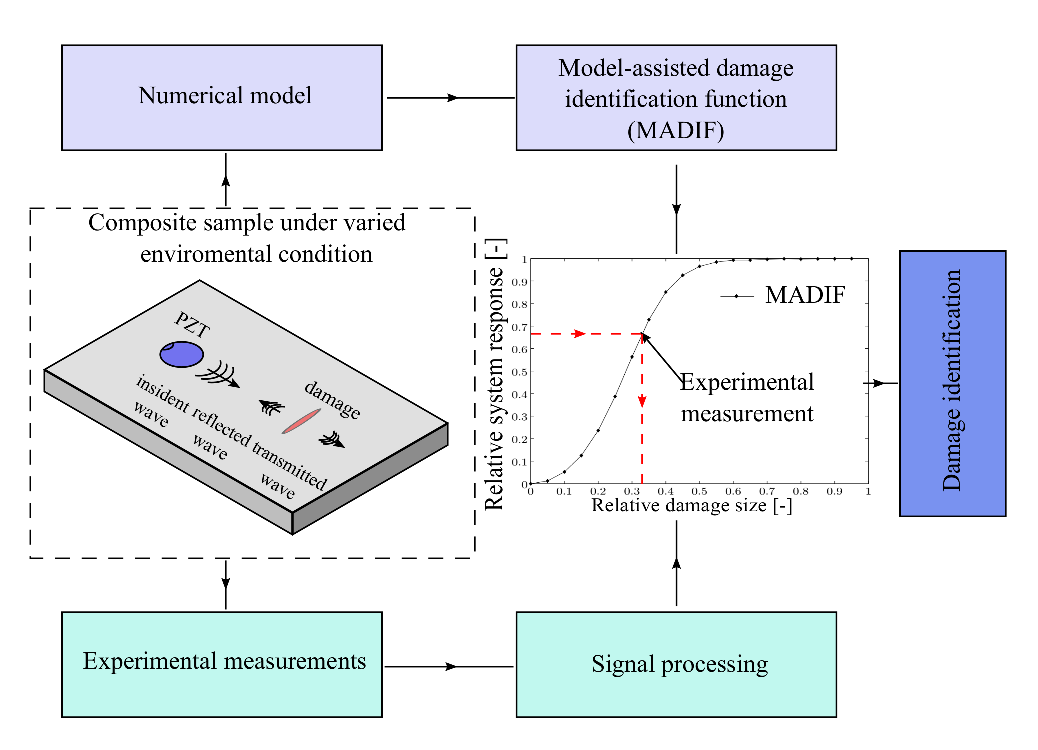
\includegraphics[width=1\textwidth]{../Figures/scheme.eps}
	\caption{Scheme of damage identification based on model--assisted damage identification function (MADIF)}
	\label{fig:scheme}
\end{figure}

The following tasks must be conducted to complete the assumed goals: 
\begin{itemize}
	\item Propose a robust numerical model of the propagating GW in the composite structure under varied ambient temperature and different boundary conditions,
	\item Experimental validation of the obtained numerical results,
	\item Determination of the model--assisted damage identification function (MADIF) to define damage influence on the propagating waves,
	\item Experimental investigation of the inspected structure,
	\item Propose a framework the damage detection based on MADIF.
\end{itemize}
\section{Significance of the project}
Currently, researchers have been focused on using a numerical modelling for development and validation of SHM techniques. The SEM was systematically implemented for simulation of elastic waves propagation in various structures, such as rods, beams, plates, etc. Moreover, an electromechanical coupling was realised for modelling the wave excitation/sensing by the piezoelectric transducers. The crucial issue is an adhesive layer between the transducer and the host structure because it transfers stresses and strains from/to the sensor. Taking into consideration the adhesive layer modelled by three--dimensional (3D) elements significantly decrease the required time increment, because its thickness is much lower than the dimensions of the remaining components. On the other hand, neglecting the adhesive layer causes that the system response is underestimated. Recently, that issue is under investigation in the work of the project leader.

\textbf{The novelty of the proposed study} can be briefly summarised as follows:
\begin{itemize}
	\item A new approach for damage identification according to the DIF defined by the numerical simulation;\\
		In this proposal, the numerical model is an inherent part of the framework of the damage identification in opposite to many methods available in the literature which rely on experimental signals only. 
	\item A new approach for numerical modelling of the composite honeycomb sandwich panel (CHSP);\\
		The CHSP is a type of structure, which is composed of the mid--core with the geometry of honeycomb bonded between thin composite skins, e.g. carbon fiber reinforced polymer (CFRP). Nowadays, modelling of CHSP by the SEM is realised in the process of homogenisation of the honeycomb core cell which is considered as the representative volume element (RVE). Such method is inaccurate for elastic wave propagation problems. In the proposed research, the real geometry of the core will be retained, and each wall of the hexagonal cell will be modelled separately by two-dimensional spectral element. Such an approach will ensure the authentic character of propagating waves with resonant effect regarding the size of the cell. 
	\item Wave propagation under varied boundary conditions;\\
		There is an evident gap in the literature for the analysis under various boundary conditions because most often researchers assume that all edges are free. In the proposed model, different boundary conditions will be taken into account.
\end{itemize}

The proposed project undertakes fundamental safety issues regarding the application of complex composite structures. The results of the investigation will have an impact on the development of worldwide research on SHM. It is expected that a novel technique for damage severity estimation will be developed.
Additionally, the numerical model of the GW propagation in advanced materials such as CHSP under various ambient temperature and boundary conditions will be improved.
\section{Work plan}
In order to achieve the intended goals, the following research plan will be implemented:
\begin{enumerate}[label=\Roman*.]
	\item Numerical modelling of the baseline.\\
	Selection of the parameters of the simulations:
	\begin{itemize}
		\item dimension and size of elements depending on the wavelength; 
		\item duration time of propagating waves and time increment used in the explicit solver.
	\end{itemize}
	\item Experimental model validation.
	\begin{itemize}
		\item Experimental measurements at the IMP PAN laboratory.
	\end{itemize}
	\item Determination of the MADIF.
	\begin{itemize}
		\item Selection of the parameter related to damage: type, size, location, orientation;
		\item Selection of inspection method: pitch--catch, pulse--echo;
		\item Selection of the parameter related to the response of the object: the amplitude of the scattered wave, time--of--flight of the wave packet reflected from the defect;
		\item Milestone: MADIF curve.
		\end{itemize}
	\item Experimental investigation of MADIF based damage identification.
	\begin{itemize}
		\item Experimental measurements and signal processing;
		\item Localisation and quantifying the severity of damage based on MADIF;
		\item Analysis and summary of obtained results.
	\end{itemize}
\end{enumerate}

The crucial issue to successfully implement the plan mentioned above is the accurate and robust model to perform a large number of numerical simulations. The solution would be using two--dimensional (2D) elements instead of full 3D implementation or a mix of 2D and 3D elements (i.e. for piezoelectric transducers only). Moreover, computation speedup will be achieved by using parallel calculation on the multi--core graphics processing unit (GPU).

\section{Methods of research}
The numerical modelling of the GW propagation is a complex and challenging process due to the multimodal and dispersive character of this phenomenon. The appropriate modelling technique should be adaptable to the different types of structure, accurate and time efficient. The SEM is one of the methods, which was successfully implemented and fulfils conditions mentioned above. This method, which was developed by Patera \cite{patera1984spectral}, combines the flexibility of finite element method (FEM) and fast convergence of spectral methods in the frequency domain. The SEM is well known to the leader of the project \cite{fiborek2018time, sikdar2018effects} and the leader’s supervisor who is a worldwide expert in the field of modelling the elastic wave propagation phenomenon \cite{kudela2007modelling,kudela20093d,kudela2016parallel} and SHM \cite{ostachowicz2009damage}.

Numerical modelling of the CHSP usually is realised by the homogenization of material properties. Unfortunately, homogenization causes that the phenomenon of propagation of elastic waves in such structure is often represented with not enough details. Model based on the 3D theory of elasticity significantly increases the time of computational operations and the need for operational memory, in contrast to the proposed approach. It is proposed that each wall of the hexagonal cell is modelled separately using 2D spectral elements. The displacements of each wall are calculated in the local system and transferred into the global system through the transformation matrix. Subsequently, the core will join with the skin elements, so that displacement fields of the common geometrical points of both skin and core elements are identical. This type of connection would be implemented through the interface based on Lagrange multipliers. This approach will reduce the number of degrees of freedom in comparison to the full 3D model, which in turn will shorten the calculation time and reduce the need for operational memory.

The composite materials are used in practical applications under a wide range of the ambient temperature. Therefore, in the project, the temperature range between $-40^{\circ} C$ and $+120^{\circ} C$ will be considered. In order to perform a temperature dependent simulations, the elastic moduli of the components will be compensated \cite{sikdar2018study,sikdar2018effects} according to the methodology presented in \cite{chamis1983simplified, salamone2009guided}. Additional the changes of the remaining components, i.e. the piezoelectric transducer and the adhesive layer must be taken into consideration. The temperature characteristics of used materials are available from the manufacturers.

Moreover, during the simulations of GW the global system will be modified by imposing different essential boundary condition.

The results obtained in the simulations will be verified with the full wavefield measured by the Scanning Doppler Laser Vibrometer (SDLV) in the room temperature. But the model with the varied temperature effects will be validated in the climate chamber in the wide range of temperature (i.e. $-40^{\circ} C$ to $+120^{\circ} C$). Excitation and sensing of the waves will be conducted by the array of piezoelectric transducers attached to the samples. Necessary equipment is available in the IMP PAN laboratory.

\bibliography{../BibTeX_Preludium16}{}
\end{document}